\documentclass[10pt,aspectratio=169]{beamer}

\usetheme{CambridgeUS}
\usecolortheme{dolphin}
\setbeamertemplate{navigation symbols}{}

\usepackage{amsmath,amssymb,booktabs}
\usepackage{graphicx}
\usepackage{subcaption}

\newcommand{\system}{BriskSeed}

\title[\system]{BriskSeed: Online History-Guided Reuse for Accelerating Dynamic Approximate Nearest Neighbor Search}
\author{Hongru Gao}
\institute{Huazhong University of Science and Technology (HUST)}
\date{\today}

\begin{document}

\begin{frame}
  \titlepage
\end{frame}

\begin{frame}{Talk Roadmap (7-Step Logic)}
  \begin{enumerate}
    \item What is the problem?
    \item Why it matters?
    \item Why existing work fails?
    \item What is the key idea?
    \item What is the design?
    \item What is the experimental result?
    \item What is the takeaway?
  \end{enumerate}
\end{frame}

\begin{frame}{1) What is the Problem?}
  \textbf{Problem:}
  \vspace{0.5em}
  Graph-based ANNS suffers from heavy random memory access and cache misses, which limit search efficiency. 
  Existing acceleration techniques are mostly designed for static index snapshots and degrade under continuous 
  updates. In dynamic settings, one-shot optimization quickly becomes stale, while frequent re-optimization 
  introduces high maintenance overhead. Therefore, the key problem is how to sustain query acceleration continuously 
  under updates without hurting end-to-end throughput.
  
  i.e., Need to maximize
    \[
      \mathrm{QPS}(R)=\frac{\sum_{r=1}^{R}|\mathcal{Q}_r|}{T_s(R)+T_m(R)}
    \]
    under a recall constraint relative to baseline.

  \vspace{0.3em}
\end{frame}

\begin{frame}{2) Why it Matters?}
  \begin{itemize}
    \item ANNS is a core primitive in RAG, recommendation, anomaly detection, and fraud detection.
    \item In streaming scenarios, updates arrive continuously while decision latency budgets remain strict.
    \item Throughput decay is not just a systems issue; it can directly translate into business risk.
  \end{itemize}

  \vspace{0.6em}
  \textbf{Representative case: real-time payment fraud detection}
  \begin{itemize}
    \item Incoming transactions are embedded and matched against a continuously updated behavioral database via ANNS.
    \item The index must absorb new transactions while still serving latency-critical queries under millisecond-level SLAs.
    \item Performance degradation across updates is unacceptable because delayed retrieval can increase fraud leakage and financial loss.
  \end{itemize}

  \vspace{0.4em}
  \textbf{Empirical motivation from the paper:}
  \begin{itemize}
    \item Cross-round top-$k$ overlap is often high.
    \item Query-hit frequencies are long-tail skewed.
    \item Per-query stability is heterogeneous.
  \end{itemize}
\end{frame}

\begin{frame}{3) Why Existing Work Fails?}
  \begin{columns}[T]
    \column{0.54\textwidth}
      \small
      \textbf{Static acceleration assumptions break in dynamic workloads}
      \begin{itemize}
        \item Layout/quantization/hints are optimized for snapshots, not evolving indices.
        \item One-shot optimization gains decay as updates accumulate.
        \item Frequent global re-optimization is too expensive and hurts end-to-end QPS.
      \end{itemize}

      \vspace{0.5em}
      \textbf{Dilemma:}
      \begin{itemize}
        \item No maintenance $\Rightarrow$ stale guidance.
        \item Aggressive maintenance $\Rightarrow$ excessive overhead.
      \end{itemize}

    \column{0.46\textwidth}
      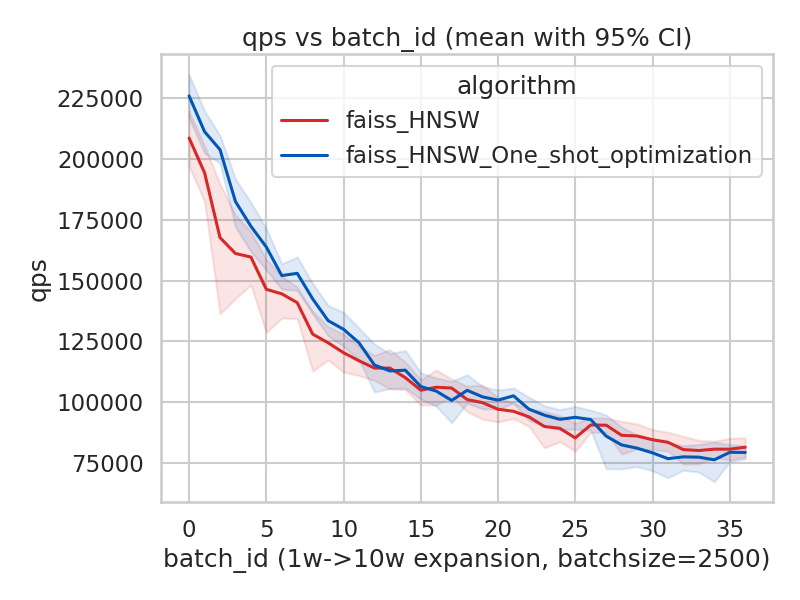
\includegraphics[width=\linewidth,height=0.32\textheight,keepaspectratio]{../figures/figure1a.png}
      \vspace{0.2em}
      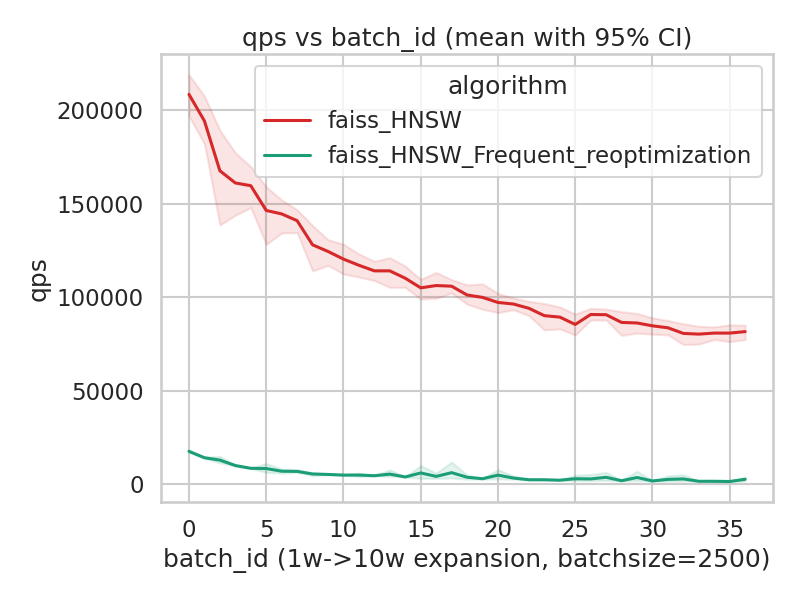
\includegraphics[width=\linewidth,height=0.32\textheight,keepaspectratio]{../figures/figure1b.png}
  \end{columns}
\end{frame}

\begin{frame}{4) What Is Our Key Idea?}
  \textbf{Turn one-shot hinting into an online reuse--validate--refresh loop.}

  \vspace{0.6em}
  \begin{itemize}
    \item Reuse past successful search outcomes as compact \textbf{seeds}.
    \item Validate reused candidates before acceptance.
    \item Refresh/evict seeds online so memory tracks workload and drift.
    \item Keep the mechanism backend-agnostic via plugin adapters.
  \end{itemize}

  \vspace{0.8em}
  \textbf{Intuition:}
  \begin{itemize}
    \item Historical outcomes are not final answers.
    \item They are warm-start guidance with bounded risk.
  \end{itemize}
\end{frame}

\begin{frame}{5) What Is the Key Design? (Architecture)}
  \begin{columns}[T]
    \column{0.6\textwidth}
      \textbf{Three co-designed layers}
      \begin{enumerate}
        \item \textbf{Seed Storage Layer}
        \begin{itemize}
          \item Two-tier memory: hot-exact + semantic-shared.
          \item Seed record: $r=\langle \mathbf{z}, n_b, \beta, \rho \rangle$.
        \end{itemize}
        \item \textbf{Seed-Guided Search Layer}
        \begin{itemize}
          \item Retrieve seed by exact key or bounded semantic probing.
          \item Recover candidates with one-hop / guarded two-hop expansion.
        \end{itemize}
        \item \textbf{Reliability Control Layer}
        \begin{itemize}
          \item Accept only if quality and consistency both pass.
          \item Otherwise immediate fallback to baseline ANN search.
        \end{itemize}
      \end{enumerate}

    \column{0.4\textwidth}
      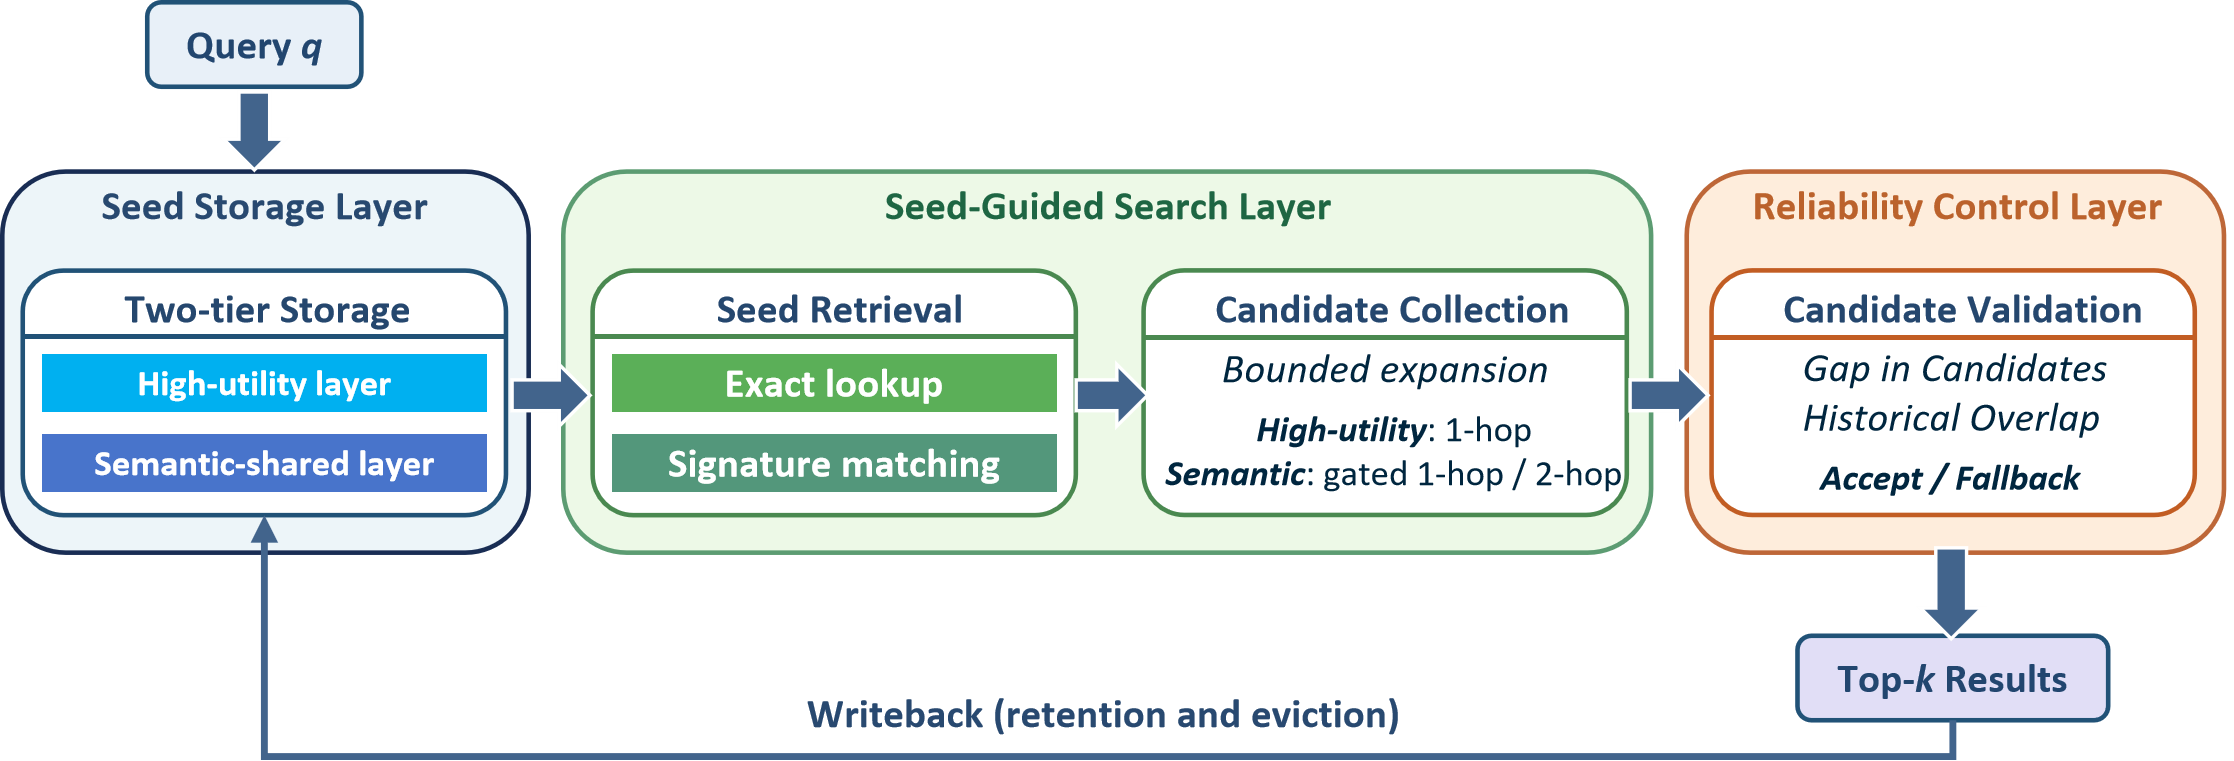
\includegraphics[width=\linewidth]{../figures/figure3.png}
  \end{columns}
\end{frame}

\begin{frame}{5) What Is the Key Design? (Pipeline and Guarantees)}
  \textbf{Bounded online pipeline per query}
  \begin{itemize}
    \item Retrieval cost: $O(Pm)$.
    \item Recovery cost: $O(kM)$ or $O(kM^2)$.
    \item Validation + writeback: bounded w.r.t. dataset size $N$.
  \end{itemize}

  \vspace{0.6em}
  \textbf{Expected latency}
  \[
    T_{\text{BriskSeed}} = T_{\text{reuse}} + (1-p_{\text{acc}})T_b,
    \quad
    T_{\text{reuse}} = O(Pm + kM^2)
  \]

  \vspace{0.4em}
  \textbf{Benefit condition}
  \[
    T_{\text{reuse}} < p_{\text{acc}}T_b
  \]

  \vspace{0.5em}
  \textbf{Consequence:} graceful degradation under drift, and speedup when reuse remains sufficiently valid.
\end{frame}

\begin{frame}{6) What Is the Experimental Result? (Placeholder)}
  \textbf{To be filled after experiments are finalized}

  \vspace{0.8em}
  \begin{itemize}
    \item Main metrics:
    \begin{itemize}
      \item End-to-end QPS across rounds
      \item Recall@$k$ vs baseline
      \item Maintenance overhead ratio
    \end{itemize}
    \item Main baselines:
    \begin{itemize}
      \item Backend native mode
      \item Existing dynamic ANNS backends (same benchmark protocol)
    \end{itemize}
    \item Ablation plan:
    \begin{itemize}
      \item Two-tier storage vs single-tier
      \item Validation on/off
      \item One-hop vs guarded two-hop
    \end{itemize}
  \end{itemize}

  \vspace{0.8em}
  \centering
  \Large \textbf{[Insert plots/tables here]}
\end{frame}

\begin{frame}{7) What Is the Takeaway?}
  \begin{itemize}
    \item Dynamic ANNS acceleration is an \textbf{efficiency-maintenance} problem, not only a search-speed problem.
    \item \system turns static hinting into \textbf{online reusable seed management}.
    \item The design is \textbf{bounded}, \textbf{reliable}, and \textbf{backend-agnostic}.
    \item Practical value: better end-to-end throughput while preserving competitive recall under continuous updates.
  \end{itemize}

  \vspace{1em}
  \centering
  \Large Thank you! \\ Questions?
\end{frame}

\end{document}
